
%% bare_conf.tex
%% V1.4b
%% 2015/08/26
%% by Michael Shell
%% See:
%% http://www.michaelshell.org/
%% for current contact information.
%%
%% This is a skeleton file demonstrating the use of IEEEtran.cls
%% (requires IEEEtran.cls version 1.8b or later) with an IEEE
%% conference paper.
%%
%% Support sites:
%% http://www.michaelshell.org/tex/ieeetran/
%% http://www.ctan.org/pkg/ieeetran
%% and
%% http://www.ieee.org/

%%*************************************************************************
%% Legal Notice:
%% This code is offered as-is without any warranty either expressed or
%% implied; without even the implied warranty of MERCHANTABILITY or
%% FITNESS FOR A PARTICULAR PURPOSE! 
%% User assumes all risk.
%% In no event shall the IEEE or any contributor to this code be liable for
%% any damages or losses, including, but not limited to, incidental,
%% consequential, or any other damages, resulting from the use or misuse
%% of any information contained here.
%%
%% All comments are the opinions of their respective authors and are not
%% necessarily endorsed by the IEEE.
%%
%% This work is distributed under the LaTeX Project Public License (LPPL)
%% ( http://www.latex-project.org/ ) version 1.3, and may be freely used,
%% distributed and modified. A copy of the LPPL, version 1.3, is included
%% in the base LaTeX documentation of all distributions of LaTeX released
%% 2003/12/01 or later.
%% Retain all contribution notices and credits.
%% ** Modified files should be clearly indicated as such, including  **
%% ** renaming them and changing author support contact information. **
%%*************************************************************************


% *** Authors should verify (and, if needed, correct) their LaTeX system  ***
% *** with the testflow diagnostic prior to trusting their LaTeX platform ***
% *** with production work. The IEEE's font choices and paper sizes can   ***
% *** trigger bugs that do not appear when using other class files.       ***                          ***
% The testflow support page is at:
% http://www.michaelshell.org/tex/testflow/



\documentclass[conference]{IEEEtran}
% Some Computer Society conferences also require the compsoc mode option,
% but others use the standard conference format.
%
% If IEEEtran.cls has not been installed into the LaTeX system files,
% manually specify the path to it like:
% \documentclass[conference]{../sty/IEEEtran}





% Some very useful LaTeX packages include:
% (uncomment the ones you want to load)


% *** MISC UTILITY PACKAGES ***
%
%\usepackage{ifpdf}
% Heiko Oberdiek's ifpdf.sty is very useful if you need conditional
% compilation based on whether the output is pdf or dvi.
% usage:
% \ifpdf
%   % pdf code
% \else
%   % dvi code
% \fi
% The latest version of ifpdf.sty can be obtained from:
% http://www.ctan.org/pkg/ifpdf
% Also, note that IEEEtran.cls V1.7 and later provides a builtin
% \ifCLASSINFOpdf conditional that works the same way.
% When switching from latex to pdflatex and vice-versa, the compiler may
% have to be run twice to clear warning/error messages.






% *** CITATION PACKAGES ***
%
%\usepackage{cite}
% cite.sty was written by Donald Arseneau
% V1.6 and later of IEEEtran pre-defines the format of the cite.sty package
% \cite{} output to follow that of the IEEE. Loading the cite package will
% result in citation numbers being automatically sorted and properly
% "compressed/ranged". e.g., [1], [9], [2], [7], [5], [6] without using
% cite.sty will become [1], [2], [5]--[7], [9] using cite.sty. cite.sty's
% \cite will automatically add leading space, if needed. Use cite.sty's
% noadjust option (cite.sty V3.8 and later) if you want to turn this off
% such as if a citation ever needs to be enclosed in parenthesis.
% cite.sty is already installed on most LaTeX systems. Be sure and use
% version 5.0 (2009-03-20) and later if using hyperref.sty.
% The latest version can be obtained at:
% http://www.ctan.org/pkg/cite
% The documentation is contained in the cite.sty file itself.






% *** GRAPHICS RELATED PACKAGES ***
%
\ifCLASSINFOpdf
  % \usepackage[pdftex]{graphicx}
  % declare the path(s) where your graphic files are
  % \graphicspath{{../pdf/}{../jpeg/}}
  % and their extensions so you won't have to specify these with
  % every instance of \includegraphics
  % \DeclareGraphicsExtensions{.pdf,.jpeg,.png}
\else
  % or other class option (dvipsone, dvipdf, if not using dvips). graphicx
  % will default to the driver specified in the system graphics.cfg if no
  % driver is specified.
  % \usepackage[dvips]{graphicx}
  % declare the path(s) where your graphic files are
  % \graphicspath{{../eps/}}
  % and their extensions so you won't have to specify these with
  % every instance of \includegraphics
  % \DeclareGraphicsExtensions{.eps}
\fi
% graphicx was written by David Carlisle and Sebastian Rahtz. It is
% required if you want graphics, photos, etc. graphicx.sty is already
% installed on most LaTeX systems. The latest version and documentation
% can be obtained at: 
% http://www.ctan.org/pkg/graphicx
% Another good source of documentation is "Using Imported Graphics in
% LaTeX2e" by Keith Reckdahl which can be found at:
% http://www.ctan.org/pkg/epslatex
%
% latex, and pdflatex in dvi mode, support graphics in encapsulated
% postscript (.eps) format. pdflatex in pdf mode supports graphics
% in .pdf, .jpeg, .png and .mps (metapost) formats. Users should ensure
% that all non-photo figures use a vector format (.eps, .pdf, .mps) and
% not a bitmapped formats (.jpeg, .png). The IEEE frowns on bitmapped formats
% which can result in "jaggedy"/blurry rendering of lines and letters as
% well as large increases in file sizes.
%
% You can find documentation about the pdfTeX application at:
% http://www.tug.org/applications/pdftex





% *** MATH PACKAGES ***
%
%\usepackage{amsmath}
% A popular package from the American Mathematical Society that provides
% many useful and powerful commands for dealing with mathematics.
%
% Note that the amsmath package sets \interdisplaylinepenalty to 10000
% thus preventing page breaks from occurring within multiline equations. Use:
%\interdisplaylinepenalty=2500
% after loading amsmath to restore such page breaks as IEEEtran.cls normally
% does. amsmath.sty is already installed on most LaTeX systems. The latest
% version and documentation can be obtained at:
% http://www.ctan.org/pkg/amsmath





% *** SPECIALIZED LIST PACKAGES ***
%
%\usepackage{algorithmic}
% algorithmic.sty was written by Peter Williams and Rogerio Brito.
% This package provides an algorithmic environment fo describing algorithms.
% You can use the algorithmic environment in-text or within a figure
% environment to provide for a floating algorithm. Do NOT use the algorithm
% floating environment provided by algorithm.sty (by the same authors) or
% algorithm2e.sty (by Christophe Fiorio) as the IEEE does not use dedicated
% algorithm float types and packages that provide these will not provide
% correct IEEE style captions. The latest version and documentation of
% algorithmic.sty can be obtained at:
% http://www.ctan.org/pkg/algorithms
% Also of interest may be the (relatively newer and more customizable)
% algorithmicx.sty package by Szasz Janos:
% http://www.ctan.org/pkg/algorithmicx




% *** ALIGNMENT PACKAGES ***
%
%\usepackage{array}
% Frank Mittelbach's and David Carlisle's array.sty patches and improves
% the standard LaTeX2e array and tabular environments to provide better
% appearance and additional user controls. As the default LaTeX2e table
% generation code is lacking to the point of almost being broken with
% respect to the quality of the end results, all users are strongly
% advised to use an enhanced (at the very least that provided by array.sty)
% set of table tools. array.sty is already installed on most systems. The
% latest version and documentation can be obtained at:
% http://www.ctan.org/pkg/array


% IEEEtran contains the IEEEeqnarray family of commands that can be used to
% generate multiline equations as well as matrices, tables, etc., of high
% quality.




% *** SUBFIGURE PACKAGES ***
%\ifCLASSOPTIONcompsoc
%  \usepackage[caption=false,font=normalsize,labelfont=sf,textfont=sf]{subfig}
%\else
%  \usepackage[caption=false,font=footnotesize]{subfig}
%\fi
% subfig.sty, written by Steven Douglas Cochran, is the modern replacement
% for subfigure.sty, the latter of which is no longer maintained and is
% incompatible with some LaTeX packages including fixltx2e. However,
% subfig.sty requires and automatically loads Axel Sommerfeldt's caption.sty
% which will override IEEEtran.cls' handling of captions and this will result
% in non-IEEE style figure/table captions. To prevent this problem, be sure
% and invoke subfig.sty's "caption=false" package option (available since
% subfig.sty version 1.3, 2005/06/28) as this is will preserve IEEEtran.cls
% handling of captions.
% Note that the Computer Society format requires a larger sans serif font
% than the serif footnote size font used in traditional IEEE formatting
% and thus the need to invoke different subfig.sty package options depending
% on whether compsoc mode has been enabled.
%
% The latest version and documentation of subfig.sty can be obtained at:
% http://www.ctan.org/pkg/subfig




% *** FLOAT PACKAGES ***
%
%\usepackage{fixltx2e}
% fixltx2e, the successor to the earlier fix2col.sty, was written by
% Frank Mittelbach and David Carlisle. This package corrects a few problems
% in the LaTeX2e kernel, the most notable of which is that in current
% LaTeX2e releases, the ordering of single and double column floats is not
% guaranteed to be preserved. Thus, an unpatched LaTeX2e can allow a
% single column figure to be placed prior to an earlier double column
% figure.
% Be aware that LaTeX2e kernels dated 2015 and later have fixltx2e.sty's
% corrections already built into the system in which case a warning will
% be issued if an attempt is made to load fixltx2e.sty as it is no longer
% needed.
% The latest version and documentation can be found at:
% http://www.ctan.org/pkg/fixltx2e


%\usepackage{stfloats}
% stfloats.sty was written by Sigitas Tolusis. This package gives LaTeX2e
% the ability to do double column floats at the bottom of the page as well
% as the top. (e.g., "\begin{figure*}[!b]" is not normally possible in
% LaTeX2e). It also provides a command:
%\fnbelowfloat
% to enable the placement of footnotes below bottom floats (the standard
% LaTeX2e kernel puts them above bottom floats). This is an invasive package
% which rewrites many portions of the LaTeX2e float routines. It may not work
% with other packages that modify the LaTeX2e float routines. The latest
% version and documentation can be obtained at:
% http://www.ctan.org/pkg/stfloats
% Do not use the stfloats baselinefloat ability as the IEEE does not allow
% \baselineskip to stretch. Authors submitting work to the IEEE should note
% that the IEEE rarely uses double column equations and that authors should try
% to avoid such use. Do not be tempted to use the cuted.sty or midfloat.sty
% packages (also by Sigitas Tolusis) as the IEEE does not format its papers in
% such ways.
% Do not attempt to use stfloats with fixltx2e as they are incompatible.
% Instead, use Morten Hogholm'a dblfloatfix which combines the features
% of both fixltx2e and stfloats:
%
% \usepackage{dblfloatfix}
% The latest version can be found at:
% http://www.ctan.org/pkg/dblfloatfix




% *** PDF, URL AND HYPERLINK PACKAGES ***
%
%\usepackage{url}
% url.sty was written by Donald Arseneau. It provides better support for
% handling and breaking URLs. url.sty is already installed on most LaTeX
% systems. The latest version and documentation can be obtained at:
% http://www.ctan.org/pkg/url
% Basically, \url{my_url_here}.




% *** Do not adjust lengths that control margins, column widths, etc. ***
% *** Do not use packages that alter fonts (such as pslatex).         ***
% There should be no need to do such things with IEEEtran.cls V1.6 and later.
% (Unless specifically asked to do so by the journal or conference you plan
% to submit to, of course. )

% correct bad hyphenation here
\hyphenation{op-tical net-works semi-conduc-tor}

% Some very useful LaTeX packages include:
% (uncomment the ones you want to load)
\usepackage{graphicx}
% declare the path(s) where your graphic files are
\graphicspath{{./figure/}}
% and their extensions so you won't have to specify these with
% every instance of \includegraphics
\DeclareGraphicsExtensions{.eps}

\usepackage{array}
\usepackage[cmex10]{amsmath}
\usepackage{mdwmath}
\usepackage{mdwtab}
\usepackage{cite}
\usepackage{placeins}
\usepackage{caption}

% *** SUBFIGURE PACKAGES ***
\usepackage[tight,footnotesize]{subfigure}
\usepackage{multirow}
\usepackage[para, flushleft]{threeparttable}

% *** ATTN *** : REMOVE HYPERREF IN FINAL SUBMISSION!
\usepackage[usenames,dvipsnames]{xcolor}
\usepackage[dvipdfm,colorlinks=false,draft=true]{hyperref}

% Latex Macros:
\newcommand{\unit}[1]{\ensuremath{\, \textrm{#1}}}
\newcommand{\unitbf}[1]{\ensuremath{\, \textrm{\bf #1}}}
\newcommand{\textsub}[2]{\ensuremath{\textrm{#1}_\textrm{#2}}}
\newcolumntype{C}[1]{>{\centering\let\newline\\\arraybackslash\hspace{0pt}}m{#1}}

%-------------------------------------------------------------------------------

\begin{document}
%
% paper title
% Titles are generally capitalized except for words such as a, an, and, as,
% at, but, by, for, in, nor, of, on, or, the, to and up, which are usually
% not capitalized unless they are the first or last word of the title.
% Linebreaks \\ can be used within to get better formatting as desired.
% Do not put math or special symbols in the title.
\title{ECE598-HH: Mobile Vital Radio \\
	Project Progress Report}


% author names and affiliations
% use a multiple column layout for up to three different
% affiliations
%\author{\IEEEauthorblockN{Michael Shell}
%\IEEEauthorblockA{School of Electrical and\\Computer Engineering\\
%Georgia Institute of Technology\\
%Atlanta, Georgia 30332--0250\\
%Email: http://www.michaelshell.org/contact.html}
%\and
%\IEEEauthorblockN{Homer Simpson}
%\IEEEauthorblockA{Twentieth Century Fox\\
%Springfield, USA\\
%Email: homer@thesimpsons.com}
%\and
%\IEEEauthorblockN{James Kirk\\ and Montgomery Scott}
%\IEEEauthorblockA{Starfleet Academy\\
%San Francisco, California 96678--2391\\
%Telephone: (800) 555--1212\\
%Fax: (888) 555--1212}}

% conference papers do not typically use \thanks and this command
% is locked out in conference mode. If really needed, such as for
% the acknowledgment of grants, issue a \IEEEoverridecommandlockouts
% after \documentclass

% for over three affiliations, or if they all won't fit within the width
% of the page, use this alternative format:
% 
\author{Amr Khasaba, Brady Salz, Junheng Zhu}

% use for special paper notices
%\IEEEspecialpapernotice{(Invited Paper)}


% make the title area
\maketitle

% As a general rule, do not put math, special symbols or citations
% in the abstract
\begin{abstract}
The intermediate report summarizes our proposal of measuring heartbeat and breathing rate by implementing frequency modulated continuous wave. We start with description of FMCW and proposed Fourier transform (FFT) based phase tracking method. Then we present our obtained experimental data demonstrating the identification of a dynamic object. We conclude the report with a to-do-list.
\end{abstract}

% no keywords
%\begin{IEEEkeywords}
%relaxation oscillator, ring oscillator, phase noise, period jitter.
%\end{IEEEkeywords}

% For peer review papers, you can put extra information on the cover
% page as needed:
% \ifCLASSOPTIONpeerreview
% \begin{center} \bfseries EDICS Category: 3-BBND \end{center}
% \fi
%
% For peerreview papers, this IEEEtran command inserts a page break and
% creates the second title. It will be ignored for other modes.
%\IEEEpeerreviewmaketitle

\section{Introduction}
\label{sec:intro}
%
% SecIntro: Introduction section
% This section mainly summarizes the project proposal/problem statement
%

For our project, we propose Mobile Vital Radio (MoViRad), a novel method of measuring physiological signals using a mobile device. We are especially interested in measuring the heartbeat and breathing rate of a person using frequency modulated continuous waves (FMCW). While past work exists that detects the breathing rate through use of a mobile device~\cite{nandakumar_mobisys15}, they were ultimately unable to get down to the fine resolution required to measure heart beats. On the other hand, the heartbeat and breathing rate detection is achieved in Vital-Radio~\cite{Adib_acm15} by extracting the heart rate based on ballistocardiography (BCG). BCG refers to body movement that is synchronous with heart beat due to ventricular pump activity; in this case, the movement of interest is the breathing, or chest movement. As a result, we expect to obtain heart beat measurement by observing small fluctuation on top of breathing. Such minute yet periodic movement could be extracted by applying Fourier transform (FFT) of the breathing signal, and identify corresponding peaks in the frequency spectrum as breathing is typically measured of sub-hertz frequency while heart beat should be in the vicinity of tens of hertz. However, Vital-Radio could not be directly applied on top of~\cite{nandakumar_mobisys15} since the medium is acoustic wave in contrast to RF signal. As a result, the sampling rate required (in other words, the frequency bin resolution of FFT) is not available. In view of the limitation presented by acoustic wave, we propose Mobile Vital Radio (MoViRad) to precisely measure the phase of received FMCW by performing interpolation on individual bins in the obtained FFT. 

The rest of the report is organized as follows. Section~\ref{sec:movirad} illustrates the development of our proposed method by presents a quick overview of FMCW followed by analysis of the FFT interpolation method. Section~\ref{sec:meas} presents the experimental data we have obtained so far. Finally, Section~\ref{sec:midreport} summarizes our progress and shows the to-do-lists to accomplish the project.

\section{Mobile Vital Radio}
\label{sec:movirad}
%
% SecMovirad: MoViRad section
%

\subsection{Background: FMCW}
\label{sec:fmcw}
During an FMCW transmission, the transmitted waveform, as shown in Fig.~\ref{fig:fmcw}, sweeps its carrier frequency linearly with respect to time between $f_{min}$ and $f_{max}$, resulting in a chirp signal being output. 

%
\begin{figure}[!htbp]
	\centering
	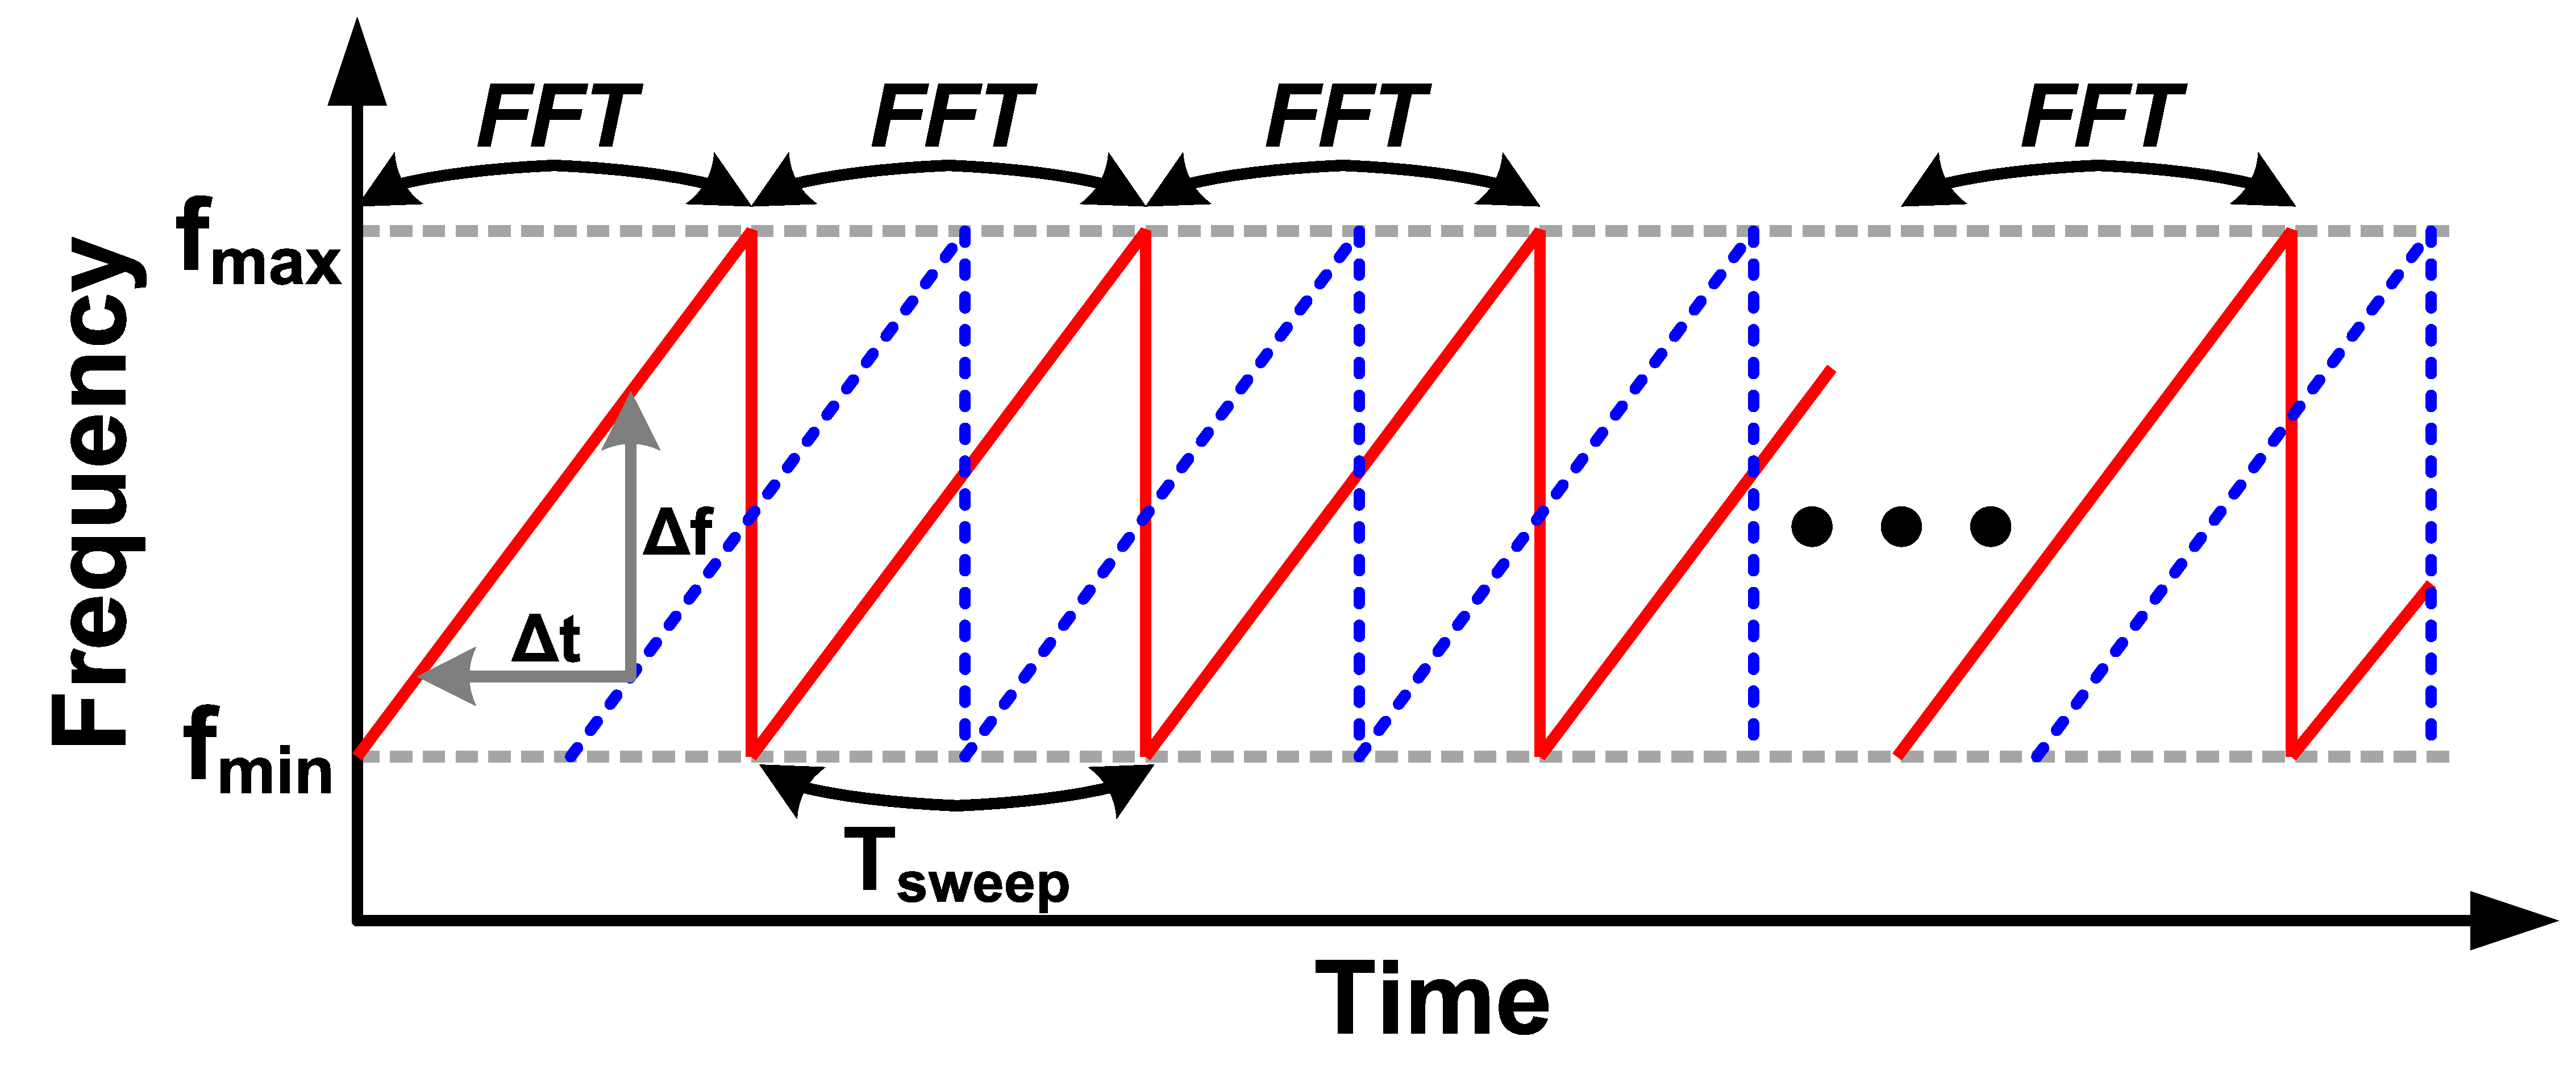
\includegraphics[width=0.9\columnwidth]{Fig01_fmcw}
	\captionsetup{justification=raggedright, singlelinecheck=false}
	\caption{Illustration of FMCW waveform.}
	\label{fig:fmcw}
\end{figure}
%

As shown in Fig.~\ref{fig:fmcw}, for instance, the red line represents the transmitted signal and the blue line represents received signal. The time delay, labeled as $\Delta t$ in the figure, is proportional related to the slope of the linear sweeping segment of the chirp. In other words, the frequency shift between transmitted and received signal could be accurately extracted from the transmission delay. Denoting the sweeping period of the chirp as $T_{sweep}$, the frequency offset $\Delta f$ can be calculated as:

%
\begin{equation}
	\label{eqn:fmcw_df}
	\Delta f = \dfrac{f_{max} - f_{min}}{T_{sweep}} \cdot \Delta t
\end{equation}
%

and the delay could be measured as:

%
\begin{equation}
	\label{eqn:fmcw_dt}
	\Delta t = \dfrac{2 \cdot d}{v_{wave}}
\end{equation}
%

where $d$ denotes the distance between transmitter and the object under test, and $\rm v_{wave}$ is the propagation velocity of the wave.

Consequently, in order to measure minute distance change such as breathing, we could send a signal towards the person so that we could back calculate the periodic chest movement associated with the breathing. Similar to the processing demonstrated in~\cite{Adib_acm15,nandakumar_mobisys15}, we apply FFT on the received signal and the perform peak search for the breathing signal. Assuming that acoustic wave travels at speed of 340m/sec at room temperature, the accuracy that we are able to achieve is roughly 2cm given that the mobile phone's microphone has a sampling rate of 44.1kHz.

\subsection{FFT Interpolation}
\label{sec:fftinterp}
While 2cm resolution is adequate for breathing, we are not able to recover heart beat signal which may only cause the chest to move in the order of millimeter. Hence, we proposed a novel interpolation method on the FFT peak search to improve the achievable accuracy. The interpolation of FFT peak is performed as follows:

%
\begin{enumerate}
	\item Perform a peak search in the correct "bucket" given a pre-knowledge of the estimated frequency, and assume only one peak resides in the frequency range of interest.
	\item Since the peak is very unlikely to fall exactly in one bin, we interpolate the peak and the second largest value to find a precise phase offset using the FFT. Interpolation revolves around the two consecutive FFT samples based on the initial peak search result. Denote the peak index with $\rm k$, and the next highest peak index with $\rm k + 1$. By taking the ratio of two consecutive samples, we wil find a ratio $\rm R$:
	
	%
	\begin{equation}
		\label{eqn:ratio}
		R = \dfrac{X[k]}{X[k+1]} = \dfrac{1 - r e^{-\frac{j2\pi}{N}}}{1 -r}
	\end{equation}
	%

	where $\rm r = e^{\frac{j2\pi\delta}{N}}$ is the frequency shift, and $\rm \delta$ is our fine frequency offset. In other words, we can now solve for $r$ now as a function of $R$, and extract the phase information from that.
	\item Use the previously mentioned coarse tracking plus the additional fine tracking to get precise distance measurements
\end{enumerate} 
%

It is worth notice that the proposed interpolation method revolves around the definition of the FFT, and the fine resolution is guaranteed with appropriately selected sweep frequency ($f_{min}$ and $f_{max}$) of the chirp signal. For this project, we sweep the signal from 10kHz to 20kHz with a sweep time of 50ms, targeting a maximum distance of 2m, we can achieve a distance measurement with a maximum error of 0.25mm. Also, this method could be applied to identify multiple people simultaneously if they are separated sufficiently for our course FFT to resolve ($>$2cm). In presence of three signals, assuming each 5cm apart distance, we are able to extract three distinct peak from the received signals while still maintaining a maximum error of 7.2mm.

For the above analysis, we have assumed that only one peak reside in the frequency spectrum of interest. However, in practice, it may occur that multiple peaks of comparative power are identified within the same frequency range. Under such condition, our coarse FFT cannot resolve them individually, resulting in large errors for further analysis. For this project, we will be focusing on demonstrating the feasiblity of implementing Vital-Radio idea~\cite{Adib_acm15} using mobile phone. So the testing is conducted to ensure only one moving object at presence.







\section{Experimental Results}
\label{sec:meas}
%
% SecMeas: Experimental results
%

In this section, we presents our experimental results obtained so far. While the ultimate goal is to implement Mobile Vital Radio on cell phone, at the current phase of the project we are transmitting signal using laptop's speaker and receiving signal using cell phone. The FFT is performed using MATLAB by uploading the audio files of transmitted and received signals to the laptop. In order to correctly start the peak search, we need to first run a cross-correlation between the transmission and reception since we are currently employing two different devices. Based on the correlation result, we are able to identify the starting point of our FFT.

%
\begin{figure}[!htbp]
	\centering
	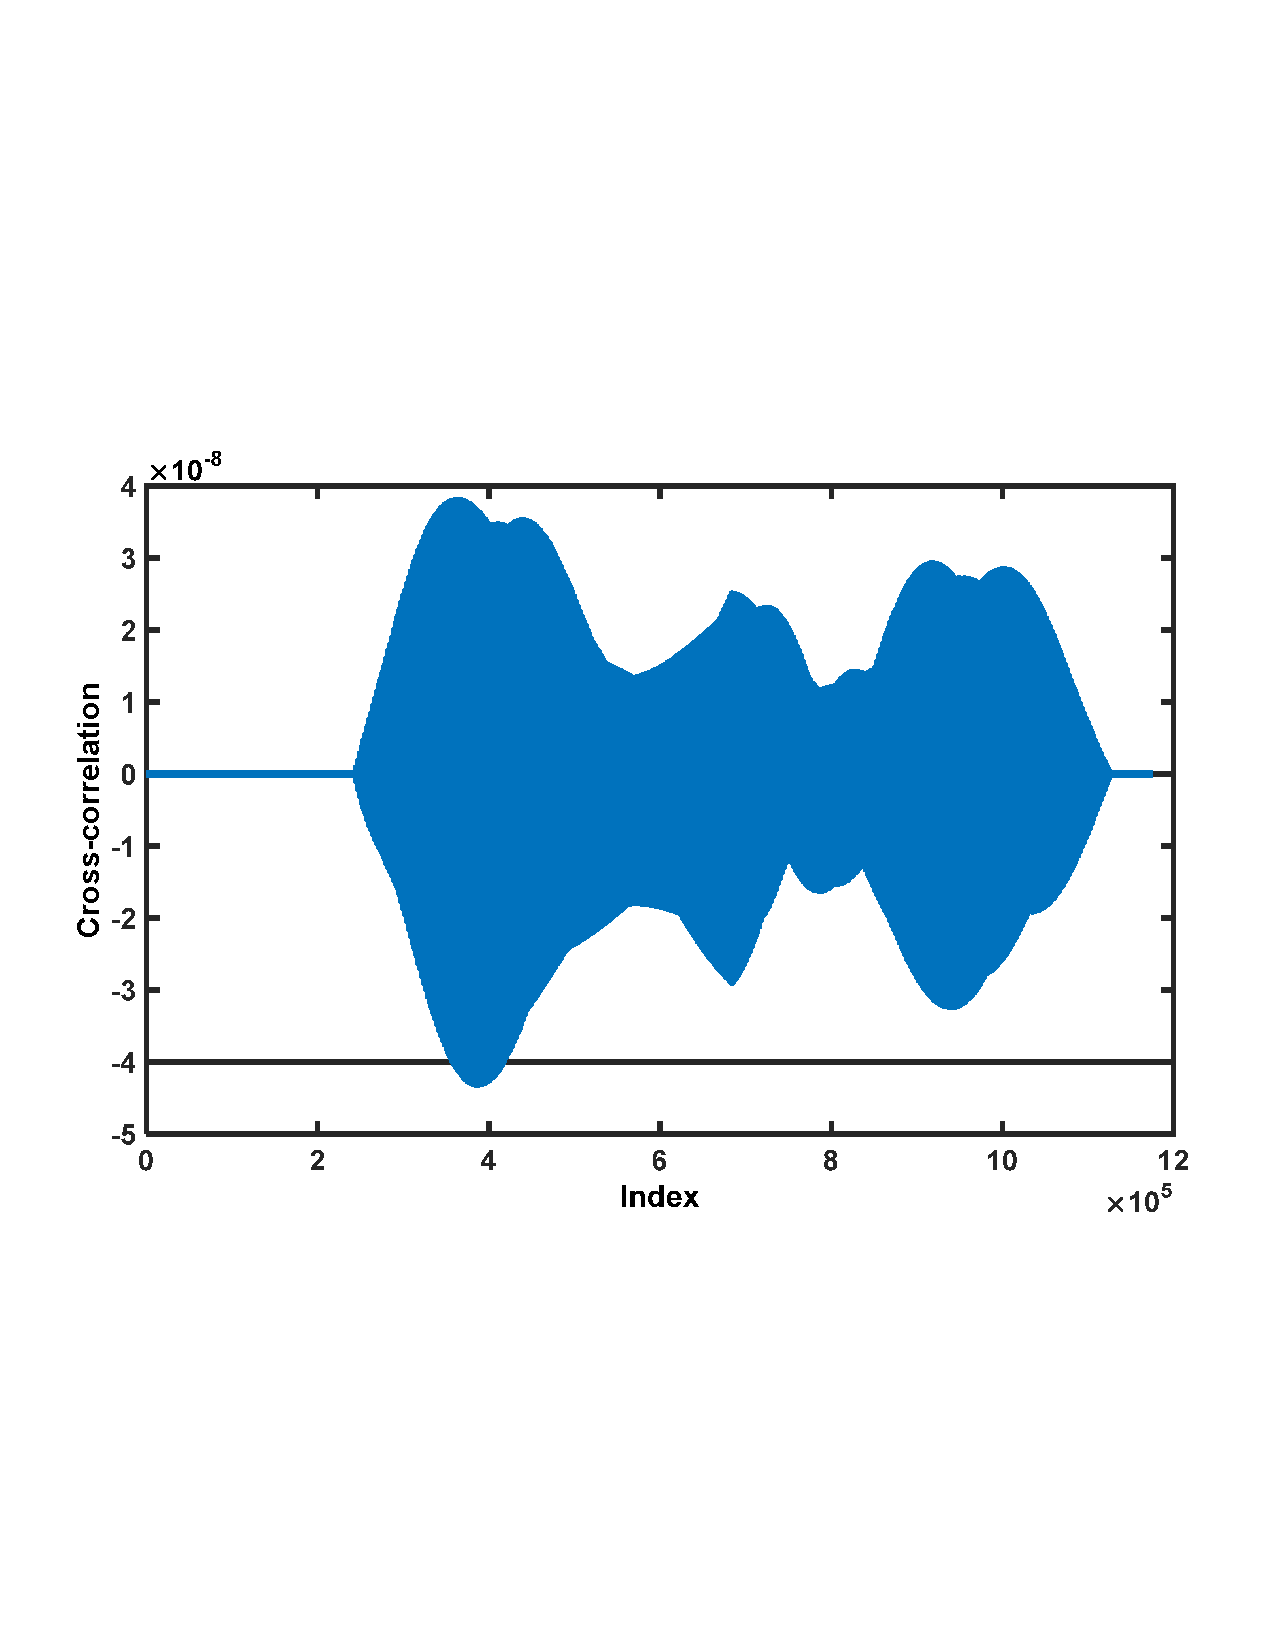
\includegraphics[width=0.9\columnwidth]{Fig02_corr}
	\captionsetup{justification=raggedright, singlelinecheck=false}
	\caption{Cross-correlation between transmitted and received signal of FMCW transmission.}
	\label{fig:corr}
\end{figure}
%

As shown in Fig.~\ref{fig:corr}, the cross-correlation of the two audio files does not show a peak indicating the index shift required corresponding to the distance offset between our position of speaker and microphone. Instead, the obtained cross-correlation actually shows amplitude-modulated waveform, which we believe is caused due to the sampling frequency offset between the two devices. In order to resolve such discrepancy between hardwares, we decide to first design an android application that is able to access both the microphone and speak of the cell phone so that the testing setup could be conducted using cell phone only. 

Next, we tested the possibility to identify static and dynamic object (assuming only one at presence) in the environment. For this experiment, we run the peak search and choose the first five peaks identified in the spectrum. As shown in Fig.~\ref{fig:path}, we are able to correctly identify the movement of the object (data 5 in the plotted figure). Small fluctuations are observed due to the fact that we have to manually press the recording and move away from the cell phone to prevent further disturbance. However, such action may still result in unnecessary noise in the process. We hope to address the issue with the android application.

%
\begin{figure}[!htbp]
	\centering
	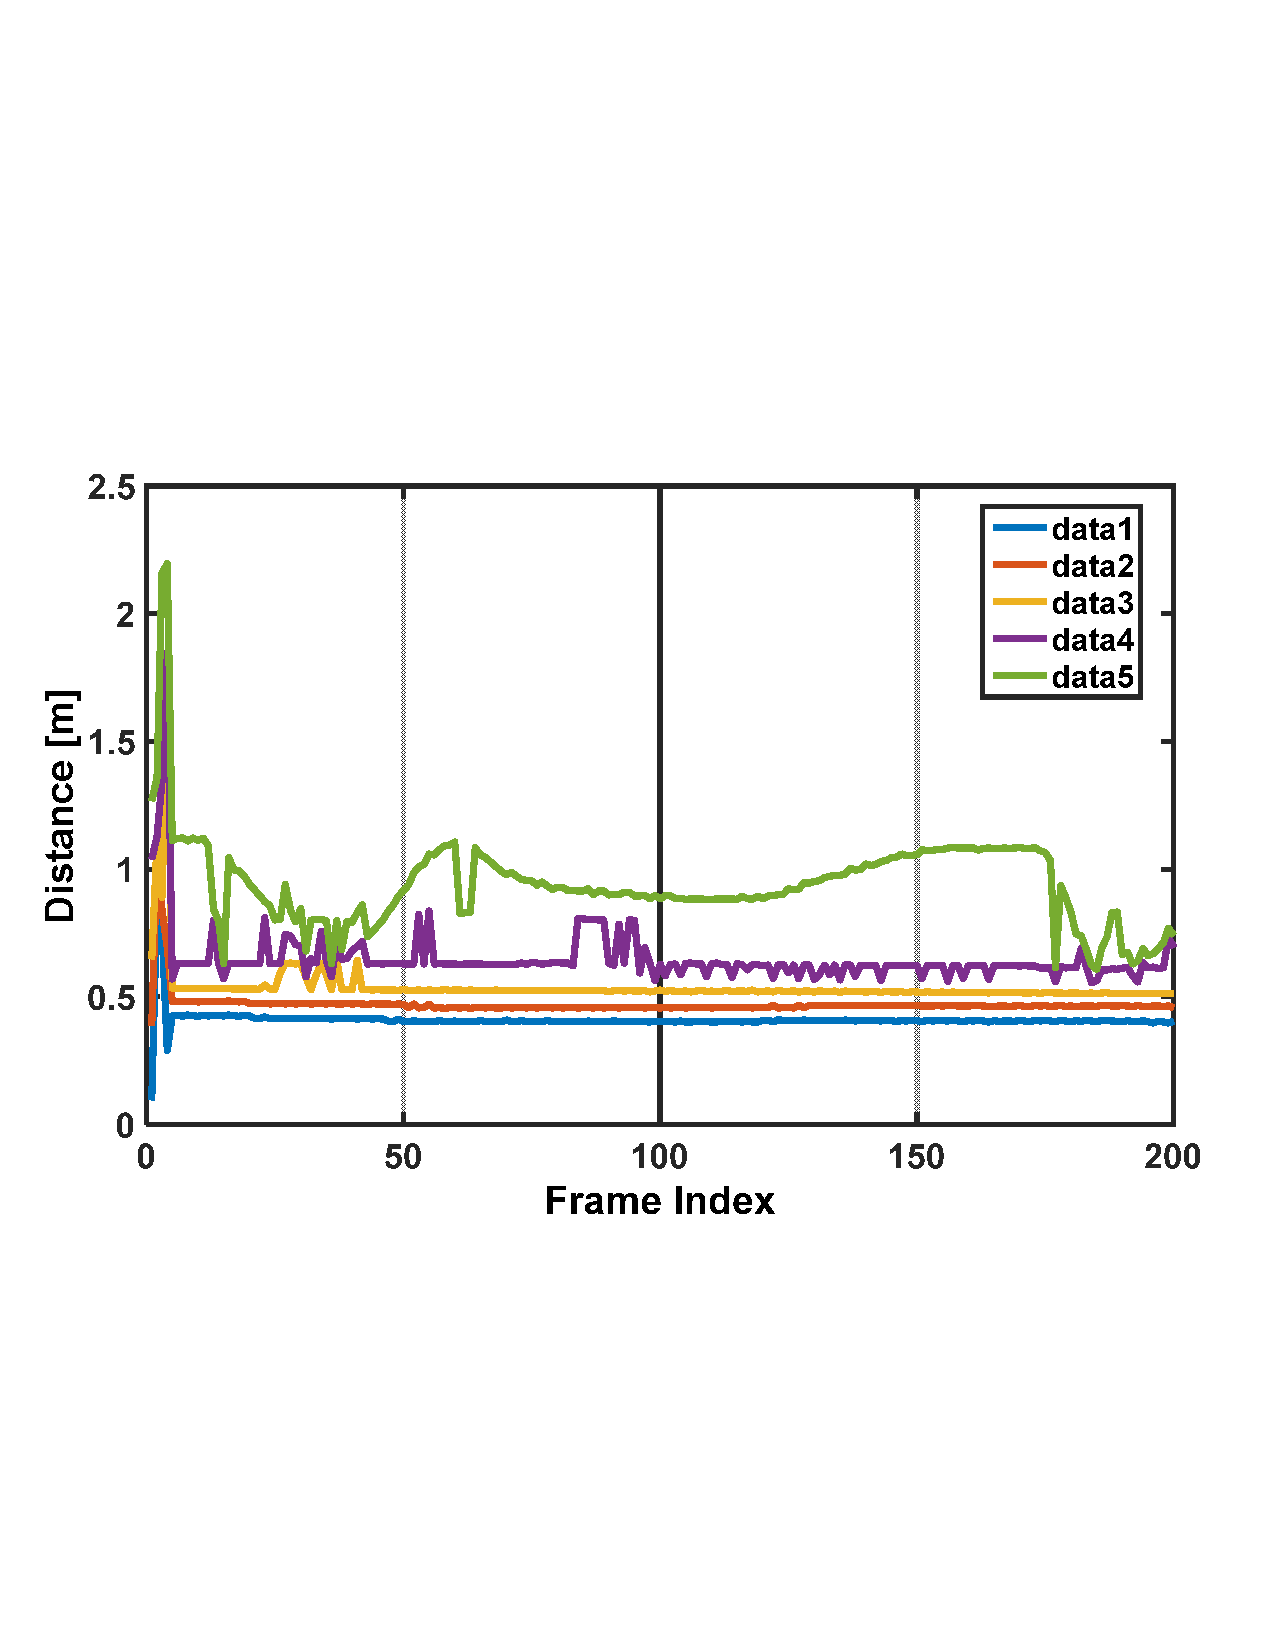
\includegraphics[width=0.9\columnwidth]{Fig03_path}
	\captionsetup{justification=raggedright, singlelinecheck=false}
	\caption{Path profile demonstrates that we are able to identify static and dynamic object in the environment.}
	\label{fig:path}
\end{figure}
%





% An example of a floating figure using the graphicx package.
% Note that \label must occur AFTER (or within) \caption.
% For figures, \caption should occur after the \includegraphics.
% Note that IEEEtran v1.7 and later has special internal code that
% is designed to preserve the operation of \label within \caption
% even when the captionsoff option is in effect. However, because
% of issues like this, it may be the safest practice to put all your
% \label just after \caption rather than within \caption{}.
%
% Reminder: the "draftcls" or "draftclsnofoot", not "draft", class
% option should be used if it is desired that the figures are to be
% displayed while in draft mode.
%
%\begin{figure}[!t]
%\centering
%\includegraphics[width=2.5in]{myfigure}
% where an .eps filename suffix will be assumed under latex, 
% and a .pdf suffix will be assumed for pdflatex; or what has been declared
% via \DeclareGraphicsExtensions.
%\caption{Simulation results for the network.}
%\label{fig_sim}
%\end{figure}

% Note that the IEEE typically puts floats only at the top, even when this
% results in a large percentage of a column being occupied by floats.


% An example of a double column floating figure using two subfigures.
% (The subfig.sty package must be loaded for this to work.)
% The subfigure \label commands are set within each subfloat command,
% and the \label for the overall figure must come after \caption.
% \hfil is used as a separator to get equal spacing.
% Watch out that the combined width of all the subfigures on a 
% line do not exceed the text width or a line break will occur.
%
%\begin{figure*}[!t]
%\centering
%\subfloat[Case I]{\includegraphics[width=2.5in]{box}%
%\label{fig_first_case}}
%\hfil
%\subfloat[Case II]{\includegraphics[width=2.5in]{box}%
%\label{fig_second_case}}
%\caption{Simulation results for the network.}
%\label{fig_sim}
%\end{figure*}
%
% Note that often IEEE papers with subfigures do not employ subfigure
% captions (using the optional argument to \subfloat[]), but instead will
% reference/describe all of them (a), (b), etc., within the main caption.
% Be aware that for subfig.sty to generate the (a), (b), etc., subfigure
% labels, the optional argument to \subfloat must be present. If a
% subcaption is not desired, just leave its contents blank,
% e.g., \subfloat[].


% An example of a floating table. Note that, for IEEE style tables, the
% \caption command should come BEFORE the table and, given that table
% captions serve much like titles, are usually capitalized except for words
% such as a, an, and, as, at, but, by, for, in, nor, of, on, or, the, to
% and up, which are usually not capitalized unless they are the first or
% last word of the caption. Table text will default to \footnotesize as
% the IEEE normally uses this smaller font for tables.
% The \label must come after \caption as always.
%
%\begin{table}[!t]
%% increase table row spacing, adjust to taste
%\renewcommand{\arraystretch}{1.3}
% if using array.sty, it might be a good idea to tweak the value of
% \extrarowheight as needed to properly center the text within the cells
%\caption{An Example of a Table}
%\label{table_example}
%\centering
%% Some packages, such as MDW tools, offer better commands for making tables
%% than the plain LaTeX2e tabular which is used here.
%\begin{tabular}{|c||c|}
%\hline
%One & Two\\
%\hline
%Three & Four\\
%\hline
%\end{tabular}
%\end{table}


% Note that the IEEE does not put floats in the very first column
% - or typically anywhere on the first page for that matter. Also,
% in-text middle ("here") positioning is typically not used, but it
% is allowed and encouraged for Computer Society conferences (but
% not Computer Society journals). Most IEEE journals/conferences use
% top floats exclusively. 
% Note that, LaTeX2e, unlike IEEE journals/conferences, places
% footnotes above bottom floats. This can be corrected via the
% \fnbelowfloat command of the stfloats package.

\section{To Do List}
\label{sec:midreport}
We are able to demonstrate that our algorithm successfully identify dynamic and static objects in the environment within a maximum distance of 2m with respect to the cell phone. As shown in Section~\ref{sec:meas}, we plan to work on the following:
\begin{enumerate}
	\item Design android app to resolve issues caused during the phase of recording itself.  
	\item More measurements with dynamic objects and move onto capturing the breathing movement.
\end{enumerate}

%\section{Acknowledgements}
%\label{sec:ack}
%This research was supported in part by Texas Instruments.



% conference papers do not normally have an appendix


% use section* for acknowledgment
%\section*{Acknowledgment}


%The authors would like to thank...





% trigger a \newpage just before the given reference
% number - used to balance the columns on the last page
% adjust value as needed - may need to be readjusted if
% the document is modified later
%\IEEEtriggeratref{8}
% The "triggered" command can be changed if desired:
%\IEEEtriggercmd{\enlargethispage{-5in}}

% references section

% can use a bibliography generated by BibTeX as a .bbl file
% BibTeX documentation can be easily obtained at:
% http://mirror.ctan.org/biblio/bibtex/contrib/doc/
% The IEEEtran BibTeX style support page is at:
% http://www.michaelshell.org/tex/ieeetran/bibtex/
%\bibliographystyle{IEEEtran}
% argument is your BibTeX string definitions and bibliography database(s)
%\bibliography{IEEEabrv,../bib/paper}
%
% <OR> manually copy in the resultant .bbl file
% set second argument of \begin to the number of references
% (used to reserve space for the reference number labels box)
%\begin{thebibliography}{1}

%\bibitem{IEEEhowto:kopka}
%H.~Kopka and P.~W. Daly, \emph{A Guide to \LaTeX}, 3rd~ed.\hskip 1em plus
%  0.5em minus 0.4em\relax Harlow, England: Addison-Wesley, 1999.

%\end{thebibliography}
\bibliographystyle{IEEEtran}
\bibliography{IEEEabrv,czbib_v1}

% that's all folks
\end{document}




